% utf-8 ru, unix eolns
\documentclass[12pt,a4paper,oneside]{extarticle}
    \righthyphenmin=2 %минимально переносится 2 символа %%%
    \sloppy

% Рукопись оформлена в соответствии с правилами оформления 
% электронной версии авторского оригинала, 
% принятыми в Издательстве МГТУ им. Н.Э. Баумана.

\usepackage{geometry} % А4, примерно 28-31 строк(а) на странице 
    \geometry{paper=a4paper}
    \geometry{includehead=false} % Нет верх. колонтитула
    \geometry{includefoot=true}  % Есть номер страницы
    \geometry{bindingoffset=0mm} % Переплет    : 0  мм
    \geometry{top=20mm}          % Поле верхнее: 20 мм
    \geometry{bottom=25mm}       % Поле нижнее : 25 мм 
    \geometry{left=25mm}         % Поле левое  : 25 мм
    \geometry{right=25mm}        % Поле правое : 25 мм
    \geometry{headsep=10mm}  % От края до верх. колонтитула: 10 мм
    \geometry{footskip=20mm} % От края до нижн. колонтитула: 20 мм 

\usepackage{cmap}
\usepackage[T2A]{fontenc} 
\usepackage[utf8x]{inputenc}
\usepackage[english,russian]{babel}
\usepackage{misccorr}

\usepackage{amsmath}
\usepackage{amsfonts}
\usepackage{amssymb}

%\usepackage{cm-super} %человеческий рендер русских шрифтов

\setlength{\parindent}{1.25cm}  % Абзацный отступ: 1,25 см
\usepackage{indentfirst}        % 1-й абзац имеет отступ

\usepackage{setspace}   

\onehalfspacing % Полуторный интервал между строками

\makeatletter
\renewcommand{\@oddfoot }{\hfil\thepage\hfil} % Номер стр.
\renewcommand{\@evenfoot}{\hfil\thepage\hfil} % Номер стр.
\renewcommand{\@oddhead }{} % Нет верх. колонтитула
\renewcommand{\@evenhead}{} % Нет верх. колонтитула
\makeatother

\usepackage{fancyvrb}

\usepackage[nounderscore]{syntax} %для поддержки рбнф
%\setlength{\grammarindent}{12em} %устанавливает нужный отступ перед ::=
\setlength{\grammarparsep}{6pt plus 1pt minus 1pt}  %сокращает расстояние между правилами

\usepackage[pdftex]{graphicx}  % поддержка картинок для пдф
\graphicspath{ {./pictures/} }
\usepackage{rotating}
%\DeclareGraphicsExtensions{.jpg,.png}

\renewcommand{\labelenumi}{\theenumi.} %меняет вид нумерованного списка

\usepackage{perpage} %нумерация сносок 
\MakePerPage{footnote}

\usepackage[all]{xy} %поддержка графов

\usepackage{listings} %листинги


\usepackage{url}


\usepackage{tikz} %для рисования графиков
\usepackage{pgfplots}


\usepackage{ccaption}%изменяет подпись к рисунку
\makeatletter 
\renewcommand{\fnum@figure}[1]{Рисунок~\thefigure~---~\sffamily}
\makeatother




\begin{document}
\pgfplotsset{compat=1.8}

\thispagestyle{empty}
\newpage
{
\centering


\textbf{
МОСКОВСКИЙ ГОСУДАРСТВЕННЫЙ ТЕХНИЧЕСКИЙ УНИВЕРСИТЕТ ИМЕНИ Н. Э. БАУМАНА \\
Факультет информатики и систем управления \\
Кафедра теоретической информатики и компьютерных технологий}
\bigskip
\bigskip
\bigskip
\bigskip
\bigskip
\bigskip
\bigskip

\vfill


Курсовой проект \\
по курсу <<Конструирование компиляторов>>

\bigskip

{\large <<Препроцессор синаксического сахара для языка Scheme>>}
\bigskip

\vfill



\hfill\parbox{4cm} {
Выполнил:\\
студент ИУ9-101 \hfill \\
Выборнов А. И.\hfill \medskip\\
Руководитель:\\
Дубанов А. В.\hfill
}


\vspace{\fill}

Москва \number\year
\clearpage
}


\tableofcontents

\clearpage

\begin{itemize}
    \item уточнить название работы
    \item что делать с тестированием
    \item
\end{itemize}

\clearpage

\section*{Введение}
\addcontentsline{toc}{section}{Введение}
    Lisp~---~это семейство динамических функциональных языков программирования.
    Первая версия языка Lisp была создана в 1958 году в ходе работ по созданию искусственного интеллекта.
    К настоящему времени сфера применения Lisp значительно увеличилась, а Lisp представляет собой целое семейство языков: Сommon Lisp, Scheme, Racket и другие. 

    В рамках работы рассматривается язык Scheme.
    Этот язык был разработан специально для учебных целей, благодаря чему включает в себя очень ограниченный, но весьма гибкий набор примитивов.
    Scheme удобен для написания скриптов и расширений~(имеется специально для этого предназначенная реализация~---~GNU Guile).

    Форматирование кода на Scheme, отслеживание парных открывающих и закрывающих скобок и некоторые другие синтаксические особенности требуют применения не слишком распространенных и привычных приложений таких как специализированная среда разработки, к примеру~---~Racket или текстовый реадактор со специальными расширениями, наиболее часто используется Emacs. 

    К числу недостатков можно также отнести: обилие скобок, затрудняющее чтение программы, отсутствие возможности записи выражений в привычном инфиксном формате.
    
    Целью данной работы является разработка и реализация функционального динамического языка на основе Scheme, который имеет более дружелюбный синтаксис.
\clearpage

\section{Теоретическая часть}
    \subsection{Scheme}
        \textcolor{red}{Поподробнее про схему.}
        В данной работе рассматривается версия языка Scheme, удолетворяющая стандарту r5rs~\cite{r5rs}.
    \subsection{Входной язык}
        \textcolor{red}{вступленние}

        Программа на исходном языке представляет собой множество определений функций.
        Переменные также рассматриваются как функции.
        Входной точкой программы является функция main.

        \textcolor{red}{подробнее про функцию main}

        \subsubsection{Токены}
            Токены языка аналогичны токенам языка программирования Scheme.
            Представлены следующие виды токенов: строка, идентификатор, число, логический тип и символ (литеральная константа). Примеры правильных токенов: 

            \begin{itemize}
                \item символ закрывающей скобки~---~\lstinline$#\)$
                \item строка~---~\lstinline$"\"r5rs\" standart\n"$
                \item идентификатор~---~\lstinline$_ident$
                \item логическая истина~---~\lstinline$#t$
                \item десятичное число~---~\lstinline$123$
                \item шестнадцатеричное число~---~\lstinline$#xDEADBEAF$
            \end{itemize}

            В рамках грамматики под нетерминалом $\langle token\rangle$ подразумевают строку, число, логический тип или символ:
            \begin{grammar}
                <token> ::= <BOOLEAN> | <NUMBER> | <CHARACTER> | <STRING>
            \end{grammar}
            Нетерминал, соответствующий идентификатору~---~<IDENTIFIER>, рассматривается отдельно.

            Единственным существенным отличием лексической структуры входного языка от Scheme является отсутствие знака перед числом, так как во входном языке знак перед числом определяется с помощью унарного минуса, который, в свою очередь, встроен в интерпретатор и фактически является элементом синтаксиса языка.
            Зависимость от регистра символов определяется настройками интерпретатора Scheme, работающем в связке с нашим компилятором.            

            Документация Sсheme~\cite{r5rs} содержит следующее определение строки в РБНФ:
            \begin{grammar}
                <string> ::= `"' <string element>* `"'

                <string element> ::= any character other than `"' or `\textbackslash' | `\textbackslash " '| `\textbackslash \textbackslash'
            \end{grammar}
            Данное определение содержит ошибку.
            Оно не позволяет определить одиночный слэш.
            Поэтому использовалось определение строки, совпадающее с таковым в реализации стандарта r5rs в рамках языка Racket. 
            \begin{grammar}
                <string> ::= `"' <string element>* `"'

                <string element> ::= any character other than `"' or `\textbackslash' | `\textbackslash " '| `\textbackslash'
            \end{grammar}

        \subsubsection{Выражения}
            Основной структурной единицей языка является выражение.
            В качестве выражения рассматриваются инфиксные операции, условный оператор и вызов функции.
            Входной язык поддерживает инфиксные операции, аналогичные операциям языка Python.
            Порядок вычислений определяется приоритетом операторов, а также может быть задан явно с помощью круглых скобок.

            Грамматика выражений в формате РБНФ:
            \begin{grammar}
                <expression> ::=
                      <expression> `**' <expression> \\
                    | <expression> (`*'|`/'|`\%'|`//') <expression> \\
                    | <expression> (`+'|`-') <expression> \\
                    | <expression> (`\textless\null\textless' | `\textgreater\null\textgreater') <expression> \\
                    | <expression> `&' <expression> \\
                    | <expression> `^' <expression> \\
                    | <expression> `|' <expression> \\
                    | <expression> `and' <expression> \\
                    | <expression> `or' <expression> \\
                    | <expression> (`\textless' | `\textless=' | `\textgreater' | `\textgreater=') <expression> \\
                    | <expression> (`==' | `!=') <expression> \\
                    | (`+'|`-') <expression> \\
                    | (`not'|`~') <expression> \\
                    | <if condition> \\
                    | <token> \\
                    | <IDENTIFIER> \\
                    | <function call> \\
                    | <lambda function call> \\
                    | `(' <expression> `)'
            \end{grammar}

            \textcolor{red}{написать про приоритеты}

            Пример выражения: \lstinline$not (x > 2 and x < 5)$.

        \subsubsection{Условия}
            В качестве условного оператора используется традиционный оператор if, который записывается в формате РБНФ следующим образом:
            \begin{grammar}
                <if condition> ::= `if' <expression> `then' <expression> `else' <expression>
            \end{grammar}
            Оператор if работает аналогично тернарному оператору: если выражение после `if' истинно, то он возвращает выражение после `then', в противном случае он возвращает выражение после `else'.

            Пример условия: \lstinline$if not (x > 2 and x < 5) then 1 else 0$.

        \subsubsection{Определение функций}
            \textcolor{red}{добавить текст}
            \begin{grammar}
                <function define> ::= `def' <IDENTIFIER> <function arguments> `=' <function body>

                <function body> ::= <function body token> (`;' <function body token>)*

                <function body token> ::= <function define> | <expression>

                <function arguments> ::= <IDENTIFIER>*
            \end{grammar}

            Пример определения функции от одного аргумента, которая возвращает модуль числа: \lstinline$def abs a = if a < 0 then -a else a$.

        \subsubsection{Анонимные функции}
            \textcolor{red}{добавить текст}
            \begin{grammar}
                <lambda function> ::= `\\' <function arguments> `->' <function body>
            \end{grammar}

            Пример анонимной функции от двух аргументов, которая находит сумму квадратов двух чисел: \lstinline$\x y-> x*x + y*y$.

        \subsubsection{Вызов функций}
            \textcolor{red}{добавить текст}

            \begin{grammar}
                <function call> ::= <IDENTIFIER> <expression>*

                <lambda function call> ::= `(' <lambda function> `)' <expression>*
            \end{grammar}

            Пример определения рекурсивной функции от одного аргумента, которая находит факториал числа: \lstinline$def fact n = if n == 0 then 1 else n*(fact n-1)$.

            Пример вызова анонимной функции от одного аргумента, который также является анонимной функцией: \lstinline$(\f -> f 3) \x->x**2$.

        \subsubsection{Импортирование символов из Scheme}
            \textcolor{red}{сначала надо реализовать}

            Пример: \lstinline${...} export a,b$
        
\clearpage

\section{Объекты и методы}
\label{sec:configuration} 
        \noindent Характеристики программного обеспечения:
        \begin{itemize}
            \item Операционная система --- Ubuntu 14.04 LTS x64.
            \item Язык программирования --- Python 2.7.3.
        \end{itemize}
        
        \noindent Характеристики оборудования:
        \begin{itemize}
            \item Процессор --- Intel Core i7-3770K 3.50 Гц 8 ядер.
            \item Оперативная память --- 16 Гбайт DDR3.
        \end{itemize}
\clearpage

\section{Реализация}
    \subsection{Используемые технологии}
        \subsubsection{ANTLR}
            что круто, а что не очень
            обязательно про минусы python версии
            особенно про различное поведение при компиляции из файла и строки %$"\""$
        \subsubsection{Graphviz}
            ...
        \subsubsection{Python unittest}
            ...
        \subsubsection{Python distutils}
            ...

    \subsection{Особенности реализации}
        общая структура:

        %входной файл -> antlr syntax tree -> AST -> lisp_tree -> lisp_file

        особоенности каждого этапа преобразования
        \subsubsection{Обработка ошибок}
            сделано
        \subsubsection{Видимость символов}
            увы нет, надо обязательно доделать
        
    \subsection{Интерфейс}
        CLI все дела

        примеры использования

        

\clearpage

\section{Тестирование}
    \textcolor{red}{что писать?}
    сравнение синтаксиса с другими языками

    \subsection{Производительность}
        График производительности от объёма нагенеренной программы.

        Это медленно.

        Для того, чтобы разобраться в чём проблема воспользуемся планировщикова cProfile и визулизатором gprof2pdf. 
        Описание что это и как использовали.

        Вуаля:

        \begin{figure}[h!]
            \center
            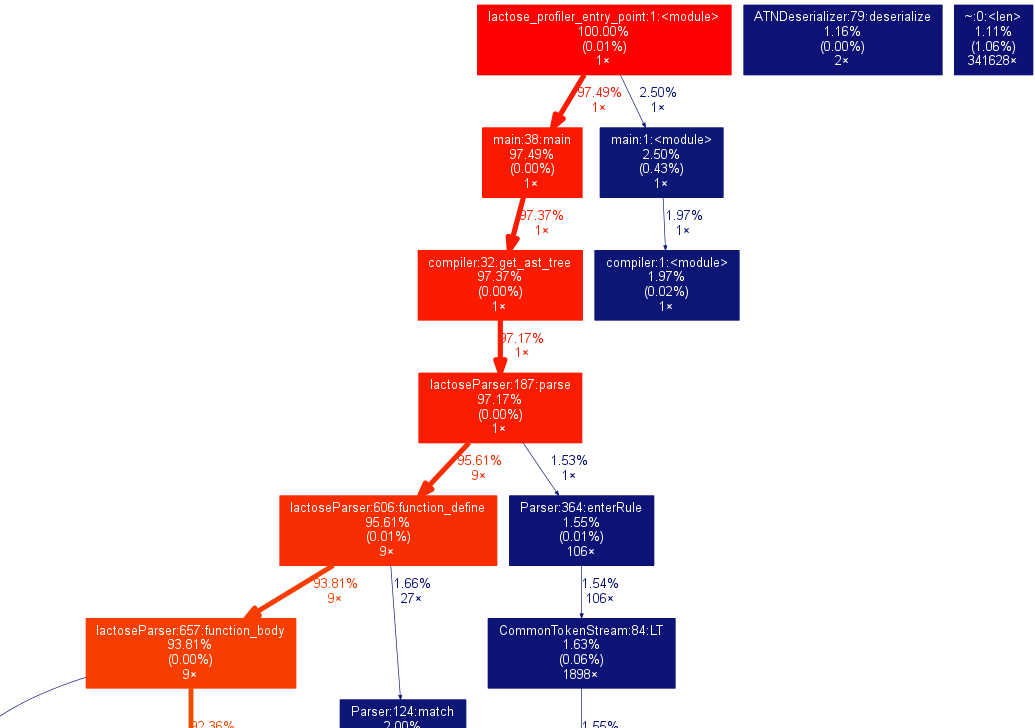
\includegraphics[scale=0.3]{lactose_stats.png}
            \caption{Результат работы профилировщика}
            \label{pic:stats}
        \end{figure}

        Вывод ANTLR для Python слоупок.
    
\clearpage

\section{Заключение}
    Что получилось. Привнесена няшность, но возможности далеко не такие как были.
\clearpage


\begin{thebibliography}{0}
\addcontentsline{toc}{section}{Список литературы}
    \bibitem{r5rs} стандарт r5rs
    \bibitem{dragon} axо ульман книга дракона
    \bibitem{antlrs} какая нибудь дока по antlr

        
\end{thebibliography}

\end{document}
